\documentclass{atistandalonetask}
\usepackage{atistandard}

\begin{document}
  \begin{atiTask}[
    title = Auslenkung einer Seite
  ]
	Eine Saite werde an ihren Enden bei $x=0$ und $x=L$ festgehalten und im Punkt $x=\frac{L}{4}$ in Richtung $y$ um den Betrag $y_0$ ausgelenkt.
	\begin{figure}[H]
	\centering
	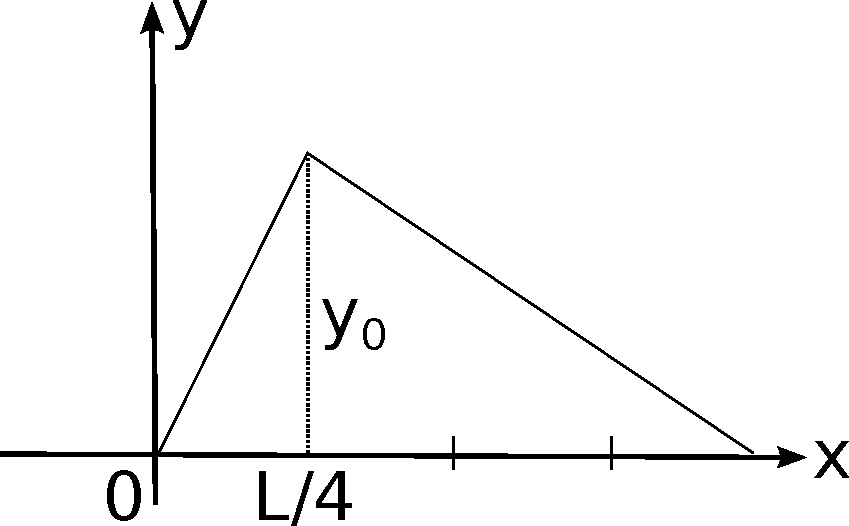
\includegraphics[width=0.70\linewidth]{picture-fourier_iv}
	\caption{Ausgelenkte Saite}
	\end{figure}

	\begin{atiSubtasks}
		\item
		Skizzieren Sie jeweils eine Fortsetzung dieser Saite für das Gebiet außerhalb des Intervalls $0\leq x\leq L$, die  \\
		(i) auf eine \textsc{Fourier}-Reihe mit der Periode $L$ führt,\\
		(ii) eine \textsc{Fourier}-Reihe erzeugt, die antisymmetrisch um $x=0$ ist,\\
		(iii) eine \textsc{Fourier}-Reihe erzeugt, die nur Cosinus-Glieder enthält.
		
		\item Geben Sie für (ii) uind (iii) jeweils die Periode und für (iii) den Wert von $a_0$ an.
		\item Berechnen Sie die \textsc{Fourier}-Reihe für (ii). 		
	\end{atiSubtasks} 
  \end{atiTask}
  \begin{atiSolution}
   Lösung folgt
   %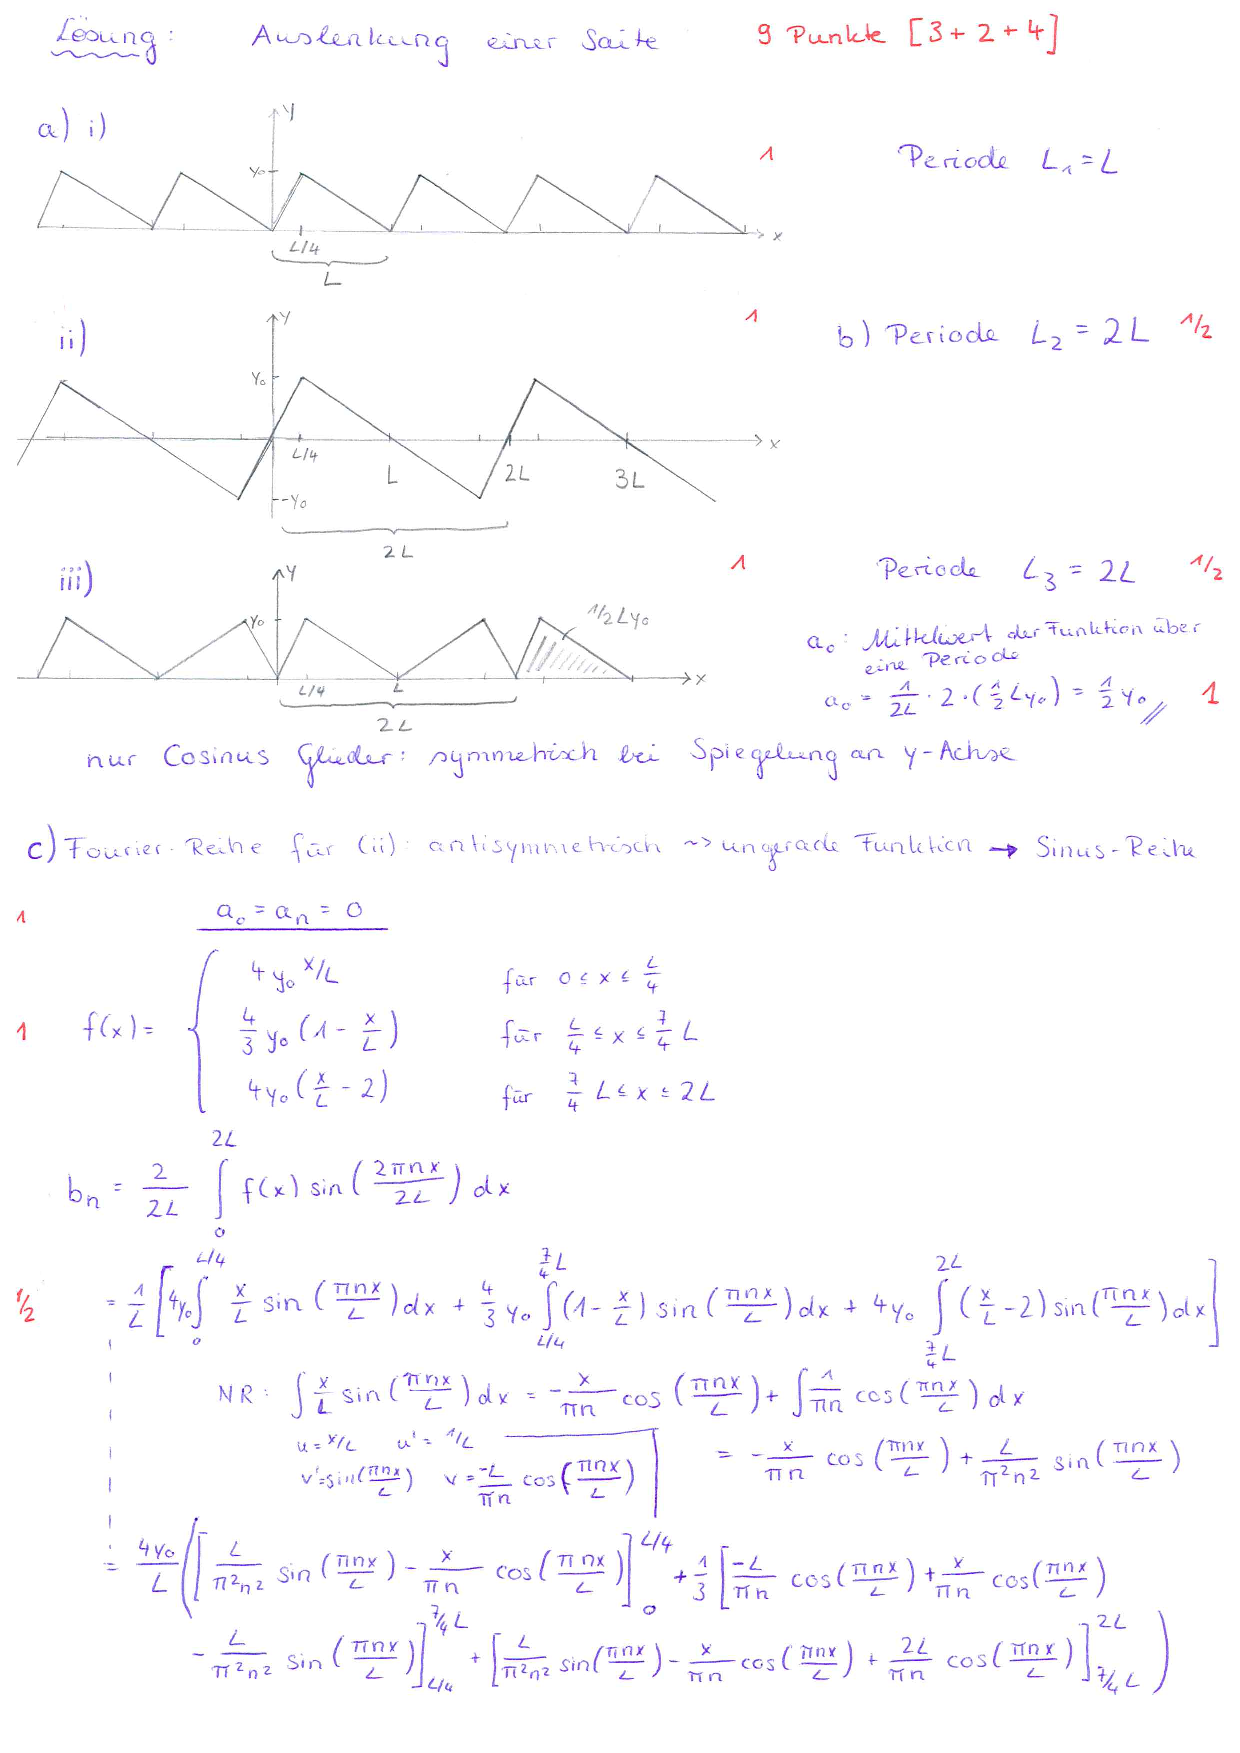
\includepdf[pages=-]{solution-fourier_iv.pdf}
  \end{atiSolution}
\end{document}